% Chapter 1

\chapter{Introducción general} % Main chapter title

\label{Chapter1} % For referencing the chapter elsewhere, use \ref{Chapter1}
\label{IntroGeneral}

En este capítulo se presenta el contexto general del trabajo final de la Maestría en Sistemas Embebidos. Se introduce el área de aplicación en la que se sitúa la máquina lanzapelotas de tenis desarrollada, se describe el sistema que se buscó automatizar y la motivación que dio origen al proyecto, se revisan soluciones comerciales y académicas existentes para esta clase de sistemas y, finalmente, se enuncian los objetivos concretos que guiaron el desarrollo del prototipo.

%----------------------------------------------------------------------------------------

% Define some commands to keep the formatting separated from the content
\newcommand{\keyword}[1]{\textbf{#1}}
\newcommand{\tabhead}[1]{\textbf{#1}}
\newcommand{\code}[1]{\texttt{#1}}
\newcommand{\file}[1]{\texttt{\bfseries#1}}
\newcommand{\option}[1]{\texttt{\itshape#1}}
\newcommand{\grados}{$^{\circ}$}

%----------------------------------------------------------------------------------------

\section{Introducción general al tema}
\label{sec:introTema}

Las máquinas lanzapelotas de tenis son equipos que permiten a un jugador practicar golpes y desplazamientos mediante el disparo programado y repetido de pelotas, sin depender de la disponibilidad de un entrenador o de un compañero de juego. Suelen combinar un mecanismo de alimentación de pelotas, motores que las impulsan a distintas velocidades y direcciones, y algún tipo de control que regula la cadencia y las características de cada lanzamiento. Su uso está extendido tanto en clubes y academias como en la práctica individual, ya que permiten sostener sesiones de entrenamiento largas y repetibles, algo difícil de lograr únicamente con la participación de otra persona.

Detrás de esta funcionalidad hay, en la mayoría de los casos, un sistema embebido: una combinación de hardware y software dedicada a controlar motores, leer sensores y coordinar el comportamiento del equipo de forma autónoma. Esta tecnología es la que permite que una máquina lanzapelotas regule la potencia y la dirección de cada disparo, detecte la presencia de pelotas y reaccione ante condiciones de falla sin intervención manual. El desarrollo de este tipo de sistemas involucra, además, restricciones propias del contexto deportivo, como la necesidad de portabilidad, de autonomía energética y de un costo razonable frente a equipos importados, lo que exige una arquitectura electrónica y de firmware pensada para operar de forma confiable en una cancha y no solo en un entorno de laboratorio.

El presente trabajo se enmarca en este contexto, con el desarrollo de un prototipo funcional de máquina lanzapelotas de tenis portátil y autónoma. La figura~\ref{fig:contextoGeneral} ilustra el lugar que ocupa el sistema desarrollado dentro de una sesión de entrenamiento típica, con el jugador, la cancha y la máquina como elementos principales del contexto de uso.

\begin{figure}[htbp]
	\centering
	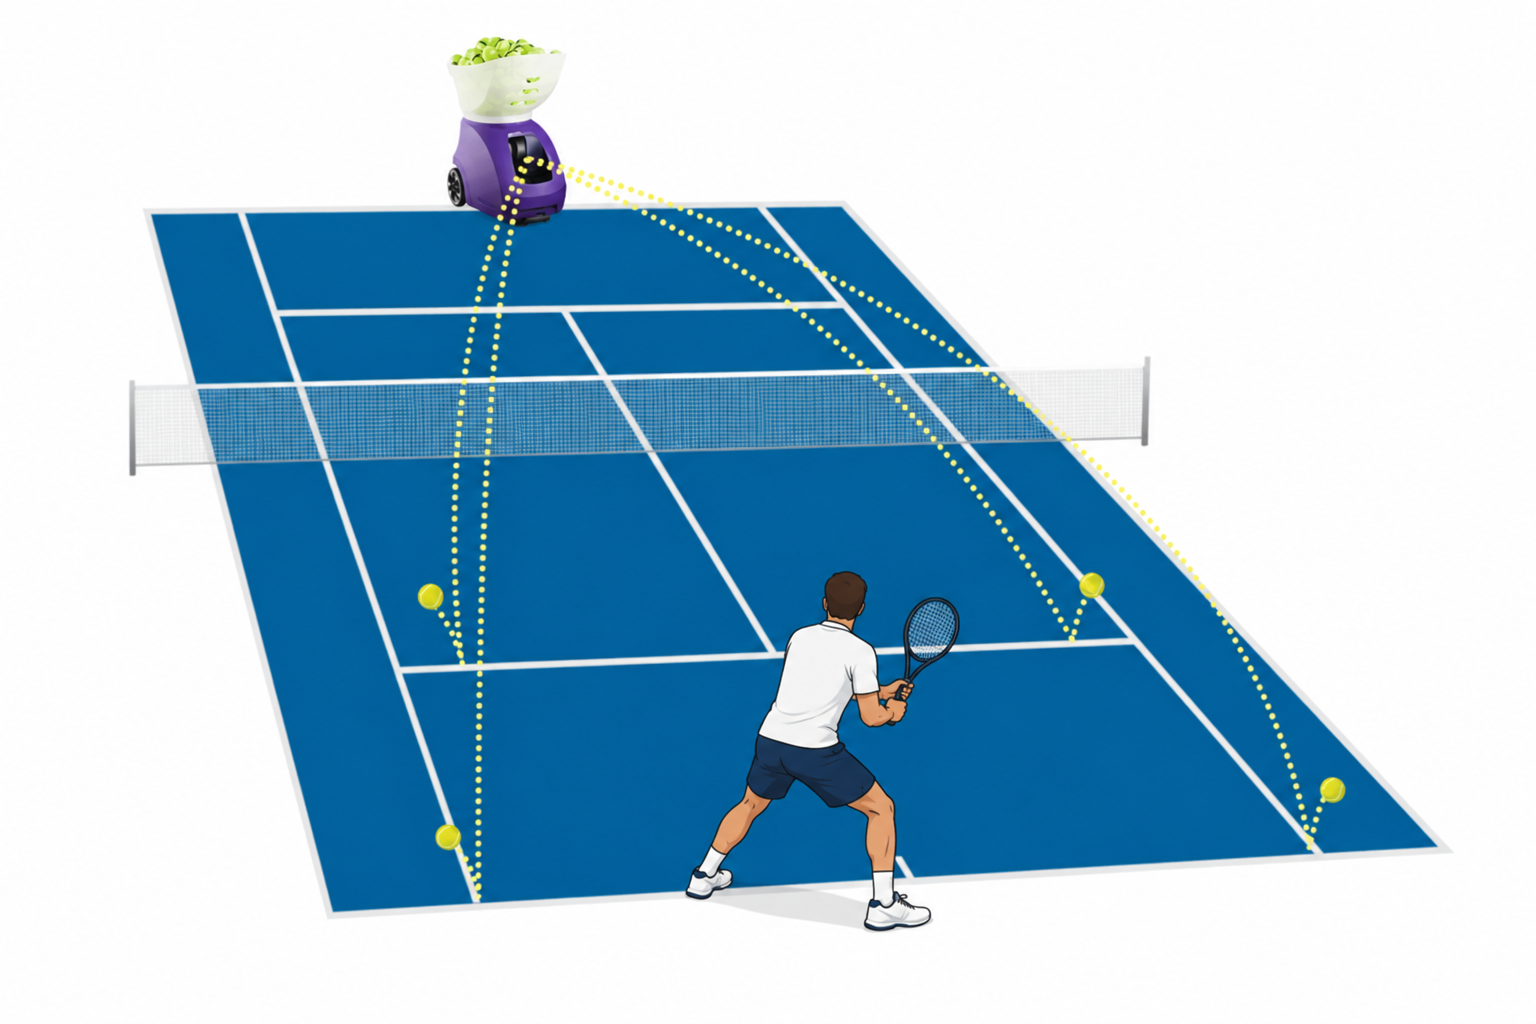
\includegraphics[width=\linewidth,keepaspectratio]{./Figures/introduccion.png}
	\caption{Ubicación de la máquina lanzapelotas dentro de una sesión de entrenamiento de tenis.}
	\label{fig:contextoGeneral}
\end{figure}

\section{Contexto y motivación}
\label{sec:contexto}

El proceso que se buscó asistir mediante este trabajo es la sesión de entrenamiento de peloteo, en la que un jugador de tenis recibe pelotas de forma sostenida para practicar golpes, desplazamientos y ritmo de juego. Habitualmente, este proceso requiere la participación de otra persona, ya sea un entrenador o un compañero, que alimente pelotas de forma manual, regule su ritmo y sostenga la sesión durante el tiempo necesario. Esta dependencia limita la disponibilidad de la práctica a los horarios y a la disposición de un segundo participante, y dificulta la repetición controlada de un mismo ejercicio a lo largo de varias sesiones.

Una máquina lanzapelotas automatiza este proceso al reemplazar a la persona que alimenta las pelotas por un mecanismo capaz de posicionarse, sostener una cadencia de disparo y regular la potencia de lanzamiento de forma programable. La motivación central de este trabajo fue disponer de un sistema de estas características que resultara portable, reproducible y económicamente accesible, en contraposición a las máquinas comerciales existentes, que suelen ser costosas, de gran tamaño y poco flexibles para su mantenimiento o modificación en el contexto local.

El desarrollo no partió de cero: existía una primera versión de la máquina que había permitido validar el concepto general de un lanzador automático de pelotas de tenis. Sin embargo, esa versión presentaba limitaciones concretas que motivaron el presente trabajo. Entre ellas se destacan un volumen y un peso elevados que dificultaban su traslado, el uso de una batería de gel pesada y de autonomía limitada, componentes electrónicos mejorables, un aprovechamiento reducido del espacio interno disponible y un sensado insuficiente para referenciar con precisión los movimientos de los mecanismos internos. Estas limitaciones impedían que el prototipo original se acercara a un producto utilizable de forma sistemática en un club o por un jugador particular.

A partir de ese diagnóstico, se planteó como motivación específica del proyecto consolidar una arquitectura de desarrollo propio en firmware, electrónica y mecánica que permitiera resolver estas limitaciones. Entre las mejoras buscadas se incluyeron la migración a baterías de litio intercambiables, la reducción del tamaño de los elementos móviles, la reorganización del ensamblaje interno y la incorporación de sensores y de finales de carrera que permitieran una referencia confiable de la posición de los mecanismos de orientación y de alimentación de pelotas. El club de tenis que colaboró con el proyecto aportó el contexto real de uso y sirvió como ámbito de referencia para validar si el sistema desarrollado resultaba de utilidad práctica para jugadores y entrenadores.

\section{Estado del arte}
\label{sec:estadoArte}

Antes de definir la arquitectura del sistema propio, se relevaron soluciones existentes para esta necesidad, tanto en el ámbito comercial como en el académico, con el fin de identificar qué características resultaban deseables y qué aspectos representaban una oportunidad de mejora.

En el ámbito comercial existe una variedad de máquinas lanzapelotas de tenis, desde modelos de gama económica orientados a jugadores individuales hasta equipos de gama alta utilizados por academias y clubes profesionales. En general, estas máquinas comparten un principio de funcionamiento similar al adoptado en este trabajo: un par de ruedas o rodillos impulsados por motores de corriente continua imprimen velocidad y efecto a la pelota, mientras que un mecanismo de alimentación regula el ritmo de disparo. Los modelos de gama más alta incorporan control remoto por aplicación móvil, memorias de programas de entrenamiento y, en algunos casos, oscilación programable en azimut para variar el punto de caída de la pelota. Sin embargo, estas soluciones presentan también limitaciones relevantes para el contexto de este proyecto. Suelen requerir importación, con los costos y los tiempos de reposición de repuestos que eso implica en la región. Además, su electrónica y su firmware son propietarios, lo que impide adaptarlos o repararlos localmente, y su costo de adquisición resulta, en general, elevado para un club o un jugador particular en comparación con un desarrollo propio basado en componentes de uso general.

En el ámbito académico y de proyectos de código abierto existen numerosos desarrollos de máquinas lanzapelotas y de robots de asistencia deportiva basados en microcontroladores de propósito general y en plataformas de bajo costo, documentados en varios casos como proyectos universitarios o de comunidades de aficionados a la electrónica. Estos desarrollos aportan evidencia de la viabilidad de construir soluciones funcionales con presupuestos acotados y, en algunos casos, exploran líneas de evolución de interés para este trabajo, como la incorporación de visión por cámara para el seguimiento del jugador o de la pelota, así como el uso de algoritmos de control más sofisticados para mejorar la precisión de la trayectoria. No obstante, se trata en general de prototipos de validación de concepto, sin un rediseño posterior orientado a la portabilidad, a la autonomía energética o a la robustez mecánica necesarias para un uso sostenido fuera de un entorno controlado. Ese es precisamente el problema que aborda la segunda iteración desarrollada en este trabajo.

De este relevamiento se desprende que el espacio no cubierto de manera satisfactoria por las soluciones existentes es el de una plataforma portátil, de desarrollo y mantenimiento locales, con un costo intermedio entre un prototipo académico de validación y una máquina comercial de gama alta. Se busca, además, una arquitectura de firmware abierta que permita evolucionar hacia funciones más avanzadas, como la incorporación futura de visión por cámara y de inteligencia artificial embebida. La tabla~\ref{tab:comparativaEstadoArte} resume las características principales relevadas para distintas categorías de soluciones existentes frente a la propuesta de este trabajo.

\begin{sidewaystable}[p]
	\centering
	\caption{Comparación de soluciones existentes para el lanzamiento asistido de pelotas de tenis.}
	\label{tab:comparativaEstadoArte}
	\scriptsize
	\setlength{\tabcolsep}{3pt}
	\renewcommand{\arraystretch}{1.2}
	\begin{tabularx}{\textheight}{|>{\raggedright\arraybackslash}X|>{\raggedright\arraybackslash}X|>{\raggedright\arraybackslash}X|>{\raggedright\arraybackslash}X|>{\raggedright\arraybackslash}X|>{\raggedright\arraybackslash}X|>{\raggedright\arraybackslash}X|>{\raggedright\arraybackslash}X|>{\raggedright\arraybackslash}X|}
		\hline
		\tabhead{Solución} & \tabhead{Controlador} & \tabhead{Memoria} & \tabhead{Conectividad} & \tabhead{Tamaño} & \tabhead{Peso} & \tabhead{Tipo de batería} & \tabhead{Autonomía} & \tabhead{Costo aprox.} \\
		\hline
		Máquina comercial gama media (WEIMILOR B0DS849RJL) & No informado por el vendedor & No informada & Control remoto y aplicación móvil & 36 cm \(\times\) 30 cm \(\times\) 50 cm & 10 kg & Litio extraíble, 24 V / 5 Ah & 2 a 4 h & \(\sim\)\$5,7 millones ARS \\
		\hline
		Máquina comercial gama alta (MINEYCHCEY PT-Smart PRO Fessional) & No informado por el vendedor & No informada; incluye 12 modos preprogramados y 28 puntos de aterrizaje & Aplicación móvil, reloj inteligente y control remoto & 43,18 cm de diámetro informado & 15 kg & Litio, 25,6 V / 6 Ah & 4 a 6 h & \(\sim\)\$11,2 millones ARS \\
		\hline
		Prototipo académico (Noguera Cundar et al., 2022) & Arduino & No informada & Control remoto por radio & No informado & No informado & LiPo recargable de 5000 mAh & No informada & No informado \\
		\hline
		Prototipo propio (este trabajo) & Microcontrolador ESP32-S3 & Juegos programables en memoria por el usuario & Bluetooth (en desarrollo) & 40 cm de diámetro aprox. & Menor que 10 kg & Baterías de litio intercambiables y extraíbles de 18 V & No determinada experimentalmente & Costo asociado a componentes impresos en 3D, motores y electrónica de uso general \\
		\hline
	\end{tabularx}
\end{sidewaystable}

\newpage
\section{Objetivos del trabajo}
\label{sec:objetivos}

A partir del diagnóstico presentado en las secciones anteriores, se definió como objetivo general desarrollar un prototipo funcional de máquina lanzapelotas de tenis portátil y autónoma que mejore la versión previa mediante un rediseño mecánico, electrónico y de firmware basado en sistemas embebidos. Con este rediseño se buscó obtener un equipo más liviano, robusto y mantenible, con mayor autonomía energética, mayor precisión en sus movimientos y una arquitectura preparada para futuras ampliaciones.

Este objetivo general se desagregó en los siguientes objetivos específicos, formulados de manera concreta y verificable:

\begin{itemize}
	\item Implementar una lógica de inicio y detención segura del equipo, de forma que la máquina pase de reposo a operación en menos de tres segundos y detenga los motores de lanzamiento y de alimentación en menos de dos segundos, tanto desde controles físicos como desde un comando remoto.
	\item Implementar una gestión de fallas que lleve al sistema a un estado seguro ante una condición anómala, impida el envío de nuevas pelotas mientras la falla persista y registre el motivo de la falla para su análisis posterior.
	\item Lograr que los ejes de altura y de orientación horizontal de lanzamiento se posicionen en el ángulo objetivo con un error absoluto máximo de $\pm 5$\grados{}, y validar la secuencia de posicionamiento antes de habilitar cada disparo.
	\item Integrar el mecanismo de alimentación de pelotas de modo que verifique la presencia de una pelota antes de cada envío y finalice el ciclo de forma segura si no hay pelota disponible dentro de un tiempo máximo definido.
	\item Permitir la configuración de al menos tres niveles de potencia de lanzamiento, de forma que el cambio de nivel impacte de manera monótona en la velocidad de salida de la pelota.
	\item Implementar una rutina de referenciación (\emph{homing}) de los ejes de altura, orientación horizontal y alimentador que permita repetir al menos diez ciclos de posicionamiento consecutivos sin pérdida de la referencia mecánica.
	\item Incorporar una aplicación móvil de control por conexión inalámbrica de corto alcance que permita iniciar y detener el equipo y configurar parámetros básicos de entrenamiento sin depender exclusivamente de los controles físicos.
	\item Validar el prototipo mediante ensayos de banco y de campo que permitan medir la repetibilidad del lanzamiento, la continuidad del mecanismo de alimentación y la estabilidad operativa del equipo, e incorporar la retroalimentación de jugadores y entrenadores que participaron de las pruebas.
\end{itemize}

Estos objetivos, junto con los criterios de aceptación asociados a cada uno, constituyen el marco de referencia utilizado a lo largo de la memoria para describir el diseño del sistema y para evaluar, en el capítulo de ensayos y resultados, en qué medida el prototipo desarrollado los alcanzó.
